\chapter{La arquitectura GPU}

\section{Introducci\'on}

Este trabajo se centra en la arquitectura GPU desarrollada por \nvidia{}, conocida como CUDA por las siglas en ingles de \textit{Compute Unified Device Architecture}.
CUDA surge naturalmente de la aplicaci\'on del hardware desarrollado para problemas gr\'aficos, pero aplicados al c\'omputo cient\'ifico.

Las placas de v\'ideo aparecen en 1978 con la introducci\'on de Intel del chip \texttt{iSBX 275}.
En 1985, la Commodore Amiga inclu\'ia un coprocesador gr\'afico que pod\'ia ejecutar instrucciones independientemente del CPU, un paso importante en la separaci\'on y especializaci\'on de las tareas.
En la d\'ecada del 90, m\'ultiples avances surgieron en la aceleraci\'on 2D para dibujar las interfaces gr\'aficas de los sistemas operativos y, para mediados de la d\'ecada, muchos fabricantes estaban incursionando en las aceleradoras 3D como agregados a las placas gr\'aficas tradicionales 2D.
A principios de la d\'ecada del 2000, se agregaron los \textit{shaders} a las placas, peque\~nos programas independientes que corr\'ian nativo en el GPU, y se pod\'ian encadenar entre s\'i, uno por pixel en la pantalla~\cite{Mark2003}.
Este paralelismo es el desarrollo fundamental que llev\'o a las GPU a poder procesar operaciones gr\'aficas \'ordenes de magnitud m\'as r\'apido que el CPU.

En el 2006, \nvidia{} introduce la arquitectura G80, que es el primer GPU que deja de resolver \'unicamente problemas de gr\'aficos para pasar a un motor gen\'erico donde cuenta con un set de instrucciones consistente para todos los tipos de operaciones que realiza (geometr\'ia, vertex y pixel shaders)~\cite{cudaHandbook}.
Como subproducto de esto, la GPU pasa a tener procesadores sim\'etricos m\'as sencillos y f\'aciles de construir.
Esta arquitectura es la que se ha mantenido y mejorado en el tiempo, permitiendo a las GPU escalar masivamente en procesadores simples, de baja frecuencia de reloj y con una disipaci\'on t\'ermica manejable.

Los puntos fuertes de las GPU modernas consisten en poder atacar los problemas de paralelismo de manera pseudo-expl\'icita, y con esto poder escalar ``f\'acilmente'' si solamente se corre en una placa con m\'as procesadores~\cite{cudaProgrammingGuide}.

T\'ecnicamente, esta arquitectura cuenta con entre cientos y miles de procesadores especializados en c\'alculo de punto flotante, procesando cada uno un \textit{thread} distinto pero
trabajando de manera sincr\'onica agrupados en bloques.
Cada procesador, a su vez, cuenta con entre $63$ a $255$ registros~\cite{NvidiaFermi,NvidiaKepler}.
Las GPU cuentas con m\'ultiples niveles de cache y memorias especializadas (subproducto de su dise\~no fundamental para gr\'aficos).
Estos no poseen instrucciones SIMD, ya que su dise\~no primario esta basado en cambio, en SIMT (\textit{Single Instruction Multiple Thread}), las cuales se ejecutan en los bloques sincr\'onicos de procesadores.
De este modo, las placas modernas como la \nvidia{} Tesla K40 alcanzan poder de c\'omputo de $4.3$ TFLOPs (4300 mil millones de operaciones de punto flotante por segundo) en c\'alculos de precisi\'on simple, $1.7$ TFLOPs en precisi\'on doble y $288$ GB/seg de transferencia de memoria, usando $2880$ CUDA Cores~\cite{NvidiaKeplerDatasheet}.
Para poner en escala la concentraci\'on de poder de c\'alculo: una computadora usando solo dos de estas placas posee una capacidad
de c\'omputo comparable a la supercomputadora m\'as potente del mundo en Noviembre 2001~\cite{Top500November2001}.
Una comparativa del poder de c\'omputo te\'orico entre GPUs y CPUs puede ver en la figura~\ref{fig:cuda-gflops}.

\begin{figure}[htbp]
    \centering
    \includegraphics[width=\plotwidthsmaller]{img/arq/cuda-gflops_ES.pdf}
    \caption{Picos te\'oricos de \performance{} en GFLOPS/s. Tomado de~\cite{cudaProgrammingGuide}.}
    \label{fig:cuda-gflops}
\end{figure}

Para poder explotar la arquitectura CUDA, los programas deben ser dise\~nados de manera de que el problema se pueda particionar usando el modelo de grilla de bloques de \threads{}.
Para este prop\'osito es que \nvidia{} desarroll\'o el lenguaje CUDA.

Hoy en d\'ia, poder aprovechar la potencialidad de las GPU requiere una reescritura completa de los c\'odigos ya existentes desarrollados para CPU y un cambio de paradigma importante, al dejar de tener vectorizaci\'on, paralelizaci\'on autom\'atica y otras t\'ecnicas tradicionales de optimizaci\'on en CPU.
Sin embargo, este trabajo ha rendido sus frutos en muchos casos: en los \'ultimos seis a\~nos, la literatura de HPC con aplicaciones en GPU ha explotado con desarrollos nuevos basados en la aceleraci\'on de algoritmos num\'ericos (su principal uso). Por este motivo, este trabajo no ahondar\'a
en las particularidades del lenguaje CUDA y su modelo de paralelismo, m\'as all\'a de lo estrictamente necesario para analizar \performance{}. Para m\'as informaci\'on se puede consultar la bibliografia~\cite{cudaHandbook,farberCuda,CudaOverview}.

Adem\'as, no todas las aplicaciones deben reescribirse de manera completa.
Con la introducci\'on de las bibliotecas \texttt{CuBLAS} y \texttt{CuFFT}, se ha buscado reemplazar con m\'inimos cambios las hist\'oricas bibliotecas \texttt{BLAS} y \texttt{FFTw}, piedras fundamentales del c\'omputo HPC~\cite{cublas,cufft}.

Nuevas soluciones para la portabilidad se siguen desarrollando: las bibliotecas como \texttt{Thrust}~\cite{thrust}, \texttt{OpenMP} 4.0~\cite{OpenMPSpec} y \texttt{OpenACC} 2.0~\cite{OpenACCSpec} son herramientas que buscan generar c\'odigo que puedan utilizar eficientemente el acelerador de c\'omputo que se haya disponible.
Estas herramientas permiten definir las operaciones de manera gen\'erica y dejan el trabajo pesado al compilador para que subdivida el problema de manera que el acelerador (CPU, GPU, MIC) necesite.
Obviamente, los ajustes finos siempre quedan pendiente para el programador especializado, pero estas herramientas representan un avance fundamental al uso masivo de t\'ecnicas de paralelizaci\'on autom\'aticas, necesarias hoy d\'ia y potencialmente imprescindibles en el futuro.

\section{Organizaci\'on de procesadores}

Los procesadores GPGPU dise\~nados por \nvidia{} han sido reorganizados a lo largo de su existencia m\'ultiples veces pero conservan algunas l\'ineas de dise\~no a trav\'es de su evoluci\'on.
A continuaci\'on se describe la organizaci\'on definida en la arquitectura \texttt{Fermi} y luego analizaremos las diferencias con \texttt{Kepler}.

Las arquitecturas de las GPUs se centran en el uso de una cantidad escalable de procesadores \textit{multithreaded} denominados \textit{Streaming Multiprocessors}~(SMs).
Un multiprocesador esta dise\~nado para ejecutar cientos de threads concurrentemente, usando sus unidades aritm\'eticas llamadas \textit{Streaming Processors}~(SPs).
Las instrucciones se encadenan para aprovechar el paralelismo a nivel instrucci\'on dentro de un mismo flujo de ejecuci\'on, y funcionando en conjunto con el paralelismo
a nivel de \thread{}, usado de manera extensa a trav\'es del hardware.
Todas las instrucciones son ejecutadas en orden y no hay predicci\'on de saltos ni ejecuci\'on especulativa, todo se ejecuta solamente cuando se lo necesita~\cite{CudaOverview}.

\begin{figure}[htb]
    \centering
    \includegraphics[width=0.5\textwidth]{img/arq/fermi-sm.pdf}
    \caption{Diagrama de bloques del SM de GF100 Fermi. Basado en~\cite{NvidiaFermi}.}
    \label{fermi_sm}
\end{figure}

Los SMs (figura~\ref{fermi_sm}) son unidades completas de ejecuci\'on.
Cada uno de ellos tiene $32$ SPs interconectados entre s\'i que operan sobre un \emph{register file} de $64$ KB com\'un a todos.
Los SMs cuentan con m\'ultiples unidades de \emph{Load/Store}, que permiten realizar accesos a memoria independientes.
Existen cuatro unidades de SFU (\textit{Special Function Unit}) por SM, para realizar r\'apidamente operaciones matem\'aticas trascendentales (trigonom\'etricas, potencias, ra\'ices, etc.).
Cada SM ejecuta simult\'aneamente una cantidad fija de threads, llamado \textit{warp}, con cada uno de estos corriendo en un SP.
Las unidades de despacho de warps se encargan de mantener registro de qu\'e \threads{} est\'an disponibles para correr en un momento dado y permiten realizar cambios de contexto por hardware
eficientemente ($<25 \mu$s)~\cite{PattersonFermi}.
Con esto, se pueden ejecutar concurrentemente dos warps distintos para esconder la latencia de las operaciones.
En precisi\'on doble, esto no es posible, as\'i que hay solamente un warp corriendo a la vez.

Un SM cuenta con una memoria com\'un de $64$ KB que se puede usar de forma autom\'atica tanto como memoria compartida com\'un a todos los \threads{} como cache L1 para todos los accesos a memoria.

\begin{figure}[htb]
    \centering
    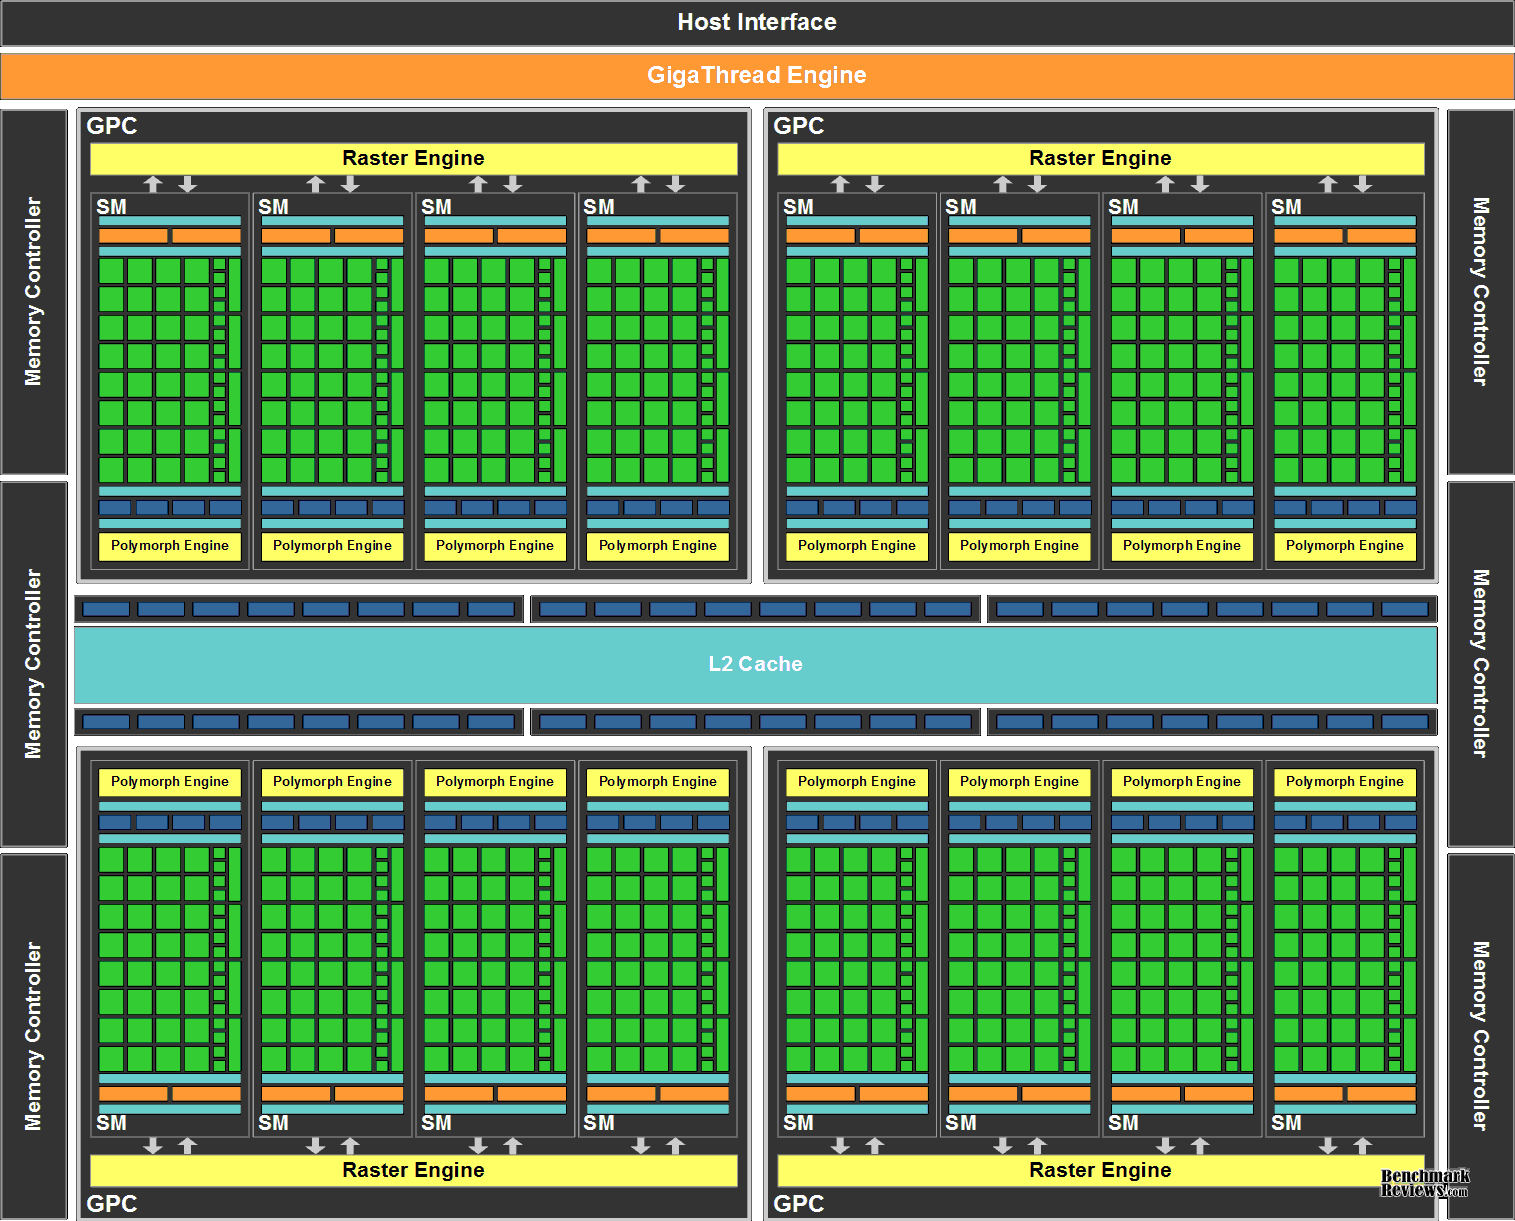
\includegraphics[width=\textwidth]{img/arq/fermi-gpu-block.pdf}
    \caption{Diagrama de bloques de GF100 Fermi. Tomado de~\cite{NvidiaFermi}.}
    \label{fermi_gpu_block}
\end{figure}

Por como funciona un pipeline gr\'afico cl\'asico, los SM se agrupan de a cuatro en GPCs (\textit{Graphics Processing Cluster}) y no interact\'ua con el modelo de c\'omputo
de CUDA.
Un esquema de esta divisi\'on global de los SM y c\'omo se comunican puede verse en la figura~\ref{fermi_gpu_block}.

%Por motivos de como funciona un pipeline gr\'afico, los SM se agrupan de 4, en un GPC (\textit{Graphics
%Processing Cluster}). Cada GPC se encarga de ejecutar los distintos pasos del pipeline gr\'afico,
%cargando a los SM con las tareas que tienen que realizar para rasterizar (es decir, convertir los
%gr\'aficos vectorialmente definidos en gr\'aficos renderizados). En aplicaciones de CUDA, estos pasos
%no importan, puesto que se trata cada SM independientemente por software.

Todos los accesos a memoria global (la memoria por fuera del procesador) se realizan a trav\'es de la cache L1 de cada SM y a trav\'es de la L2 del todo el procesador.
Esta L2 consiste de seis bancos compartidos de $128$ KB.
Estas caches se comunican de manera directa tanto con la DRAM propia de la placa como con el bus PCI Express por el cual pueden comunicarse dos placas entre s\'i, sin pasar por CPU, y son \textit{write-through}, es decir cada escritura se hace tanto en la DRAM como en la memoria cache.

%En la arquitectura Fermi, no se pueden ejecutar simult\'aneamente instrucciones de precisi\'on doble y simple y, como las de precisi\'on doble requieren ambos pipelines, suelen disminuir considerablemente el aprovechamiento de los cores.
%En la arquitectura Kepler, al usar cuatro unidades de despacho de warp, se puede elegir una mejor combinaci\'on para poder ejecutar simult\'aneamente instrucciones que no requieran usar los mismos recursos del pipeline~\cite{NvidiaKepler}.

Como estos procesadores implementan el est\'andar IEEE754-2008, cuentan con operaciones de precisi\'on simple y doble acorde al
mismo, por lo cual los c\'alculos intermedios en operaciones como FMA (\textit{Fused Multiply-Add}), que toma tres operandos y devuelve el producto de dos de ellos sumado al tercero, no pierden precisi\'on por redondeo.

%El c\'odigo escrito para CUDA se puede compilar a dos targets distintos; uno es
%el codigo binario nativo de la placa target donde se va a correr y el otro es un
%codigo intermedio, llamado c\'odigo PTX, que se JIT compila por el driver CUDA
%antes de enviar a la placa, de modo que sea portable entre placas y arquitecturas
%(retrocompatibles).

%Cuando se lanza un kernel de ejecuci\'on, este c\'odigo binario se carga en la DRAM propia
%de la placa. Este codigo va a ser ejecutado por todos los bloques que se hayan definido cuando
%se lanz\'o el kernel. El ``Thread Engine'' del GPGPU se encarga de repartir los bloques a los
%SM (Streaming Multiprocessors). Cada SM luego va a ejecutar de a grupos de 32 threads, cada uno
%de ellos corriendo sobre un SP (Streaming Processor). A traves de sus 2 o 4 unidades de dispatch de warp
%(de acuerdo a la generaci\'on de los chips), el SM puede dinamicamente cambiar el warp que se esta ejecutando en sus SP,
%escondiendo la latencia de los stalls de pipelines forzosos para la ejecucion de instrucciones de multiples clocks.
%Estos threads a su vez obtienen sus registros de un register file com\'un a todos los SP. Un scoreboard
%es mantenido por cada dispatcher de warps para poder determinar que threads estan listos para correr. En Kepler
%este scoreboard es simplificado ya que las latencias de las operaciones matem\'aticas es conocido, por
%lo cual se puede reemplazar por contadores m\'as sencillos. ~\cite{NvidiaKepler}
%Como el c\'odigo se ejecuta de manera sincr\'onica entre todos los threads del warp, las instrucciones
%condicionales proveen un problema para esta arquitectura. Como las distintas ramas del condicional
%son instrucciones excluyentes, no las deben ejecutar todos los threads simultaneamentes. El procesador
%deshabilitaba los cores que manejaban los threads de las ramas que no se ejecutaban del
%condicional~\cite{NvidiaTesla}. Para disminuir la cantidad de instrucciones de condicionales
%que se ejecutan, e cuenta con ~\cite{NvidiaFermi} predicaci\'on en todas las instrucciones de la ISA.


\section{Organizaci\'on de la memoria} \label{esquemaMemoria}

%La arquitectura CUDA esta enfocada a procesamiento de grandes cantidades de datos
%de puntos flotante. El procesador GPGPU cuenta con cientos de ALU sincronizadas
%por bloques, permitiendo un paralelismo adaptativo a distintos problemas.
%
%El procesamiento GPGPU es similar al procesamiento vectorial
%realizado por las supercomputadoras Cray y IBM que surgio en los 1960's, pero
%en vez de usar VLIW para procesamiento masivo, CUDA usa multiples hilos de ejecuci\'on
%que trabajan simultaneamente sobre los datos.
%El procesamiento consiste en un funcionamiento hibrido entre compilador y procesador. Se determina
%un conjunto de elementos a procesar y se elije de manera explicita una manera de particionar el
%problema a la hora de ser enviado para procesado a la placa.
%
%Para realizar el computo, esta arquitectura cuenta a su vez con multiples clases de memorias
%que se adaptan de maneras diferentes a los distintos procesos. Estas incluyen:

La memoria de la GPU es uno de los puntos cruciales de esta arquitectura, un esquema gr\'afico puede observarse en la figura~\ref{fig:cuda-memories}.
Esta se subdivide entre memorias on-chip y memorias on-board, de acuerdo a su ubicaci\'on y latencia de acceso, en cuatro categor\'ias distintas:

\begin{itemize}
  \item Registros
  \item Memoria local
  \item Memoria compartida
  \item Memoria global
\end{itemize}

Cada \thread{} de ejecuci\'on cuenta con una cantidad limitada de registros de punto flotante de $32$ bits con latencia de un par de ciclos de clock.
A su vez, existe una cantidad finita de registros totales que cuenta un SM (oscila entre $16535$ y $65535$ registros).
Por su baja latencia son la clase principal de almacenamiento temporal.

La memoria local es una memoria propia de cada \thread{}, y se encuentra almacenada dentro de la memoria global.
Esta memoria es definida autom\'aticamente por el compilador y sirve como \'area de almacenamiento cuando se acaban los registros: los valores anteriores se escriben a esta memoria, dejando los registros libres para nuevos valores en c\'alculos, y cuando se terminan estos c\'alculos se carga los valores originales nuevamente.
Cuenta con las mismas desventajas que la memoria global, incluyendo su tiempo de acceso.

La memoria compartida, o \textit{shared}, es una memoria que es visible para todos los \threads{} dentro de un mismo SM.
Cada \thread{} puede escribir en cualquier parte de la memoria compartida dentro de su bloque y puede ser le\'ido por cualquier otro \thread{} de este.
Es una memoria muy r\'apida, on-chip, y que tarda aproximadamente $40$ ciclos de acceso~\cite{Demystifying}.
Esta memoria es compartida con la cache L1, la cual tiene capacidad de entre $16$ KB y $64$ KB configurable por software.
Esta memoria se encuentra dividida en $32$ bancos de $2$ KB de tama\~no, permitiendo que cada uno de los $32$ \threads{} acceda independientemente a un float.
Si hubiera conflicto, los accesos a ese banco se serializar\'ian, aumentando la latencia de la llamada~\cite{farberCuda}.

La memoria global es la memoria principal fuera del chip de la GPU.
Esta es de gran tama\~no (de entre $1$ GB y $12$ GB) y es compartida por todos los SM de la GPU y los CPU que integran el sistema.
Es decir, tanto los GPU como los CPU pueden invocar las funciones de CUDA para transferir datos entre la memoria de la placa y la memoria RAM de \textit{host}.
La latencia de acceso a la memoria global es de cientos de ciclos~\cite{Demystifying}, sumamente lenta en comparaci\'on con el procesador.
La memoria global tambi\'en puede ser mapeada, o \textit{pinneada}, para que exista una copia de esa reserva tanto en la memoria en la placa como en la memoria principal del procesador. El driver de CUDA va a mantener la consistencia entre ambas de manera as\'incrona, evitando la necesidad de hacer copias de memoria expl\'icitas.
No es ilimitada la cantidad de memoria mapeada posible, por lo que es importante saber elegir qu\'e elementos se van a almacenar de esta manera.

\begin{figure}[htb]
    \centering
    \includegraphics[width=250px]{img/arq/cuda-memories_ES.pdf}
    \caption{Esquema de la jerarqu\'ia de memorias en GPU, detallando de las disponibles en cada SM, la memoria compartida (SMEN), la L2 global, la
    memoria de la placa (global) y la mapeada entre el \textit{host} y la placa de video. Tomado de~\cite{farberCuda}.}
    \label{fig:cuda-memories}
\end{figure}

Adicionalmente, la GPU cuenta con m\'ultiples niveles de memorias cache para poder aminorar el hecho de que el principal cuello de botella del c\'omputo es la latencia en los accesos a memoria global.
Estas se dividen en cuatro:

\begin{itemize}
  \item Cache L1
  \item Cache L2
  \item Cache constante
  \item Cache de textura
\end{itemize}

La cache L1 es dedicada por SM.
Esta cache fue introducida en Fermi y su dise\~no hace que tambi\'en est\'a dedicada a la memoria compartida, por lo que es posible en tiempo de ejecuci\'on darle directivas a la GPU que asigne m\'as memoria cache o m\'as memoria compartida, permitiendo a los bloques tener mayores espacios de memorias compartidas o mayores \textit{hit rates} de caches.

La cache L2 es com\'un a todos los SM de la GPU, donde, a partir de Fermi en \nvidia{}, todos los accesos de lectura y escritura a memoria global y textura pasan a trav\'es de esta~\cite{NvidiaFermi}.

La cache constante es una cache sobre la memoria global dedicada solamente a lecturas de memoria.
Esta es muy reducida (solo cuenta con $64$ KB) y est\'a optimizada para muchos accesos a la misma direcci\'on.
Cuando un \thread{} lee esta memoria, se retransmite a los dem\'as \threads{} del warp que est\'en leyendo esa misma direcci\'on, reduciendo el ancho de banda necesario.
Si, en cambio, los \threads{} leen distintas direcciones, los accesos se serializan.
Cuando hay un \emph{miss} de esta memoria, la lectura tiene el costo de una lectura de memoria global.

La cache de textura es una cache sobre la memoria global que presenta no solo localidad espacial, como la mayor\'ia de las caches de procesadores normales (es decir, la cache contiene una porci\'on consecutiva de la memoria principal),
sino que se le puede agregar el concepto de dimensiones, para poder modelar datos en m\'as de una dimensi\'on.
Esto se adapta de muy bien a los problemas de gr\'aficos en 2D y 3D, y es una herramienta clave a la hora de minimizar los accesos a matrices no solo por filas sino por columnas.
Esta cache se debe definir en momento de compilaci\'on en el c\'odigo, ya que tiene l\'imites espaciales (necesarios para poder definir \'areas de memoria sobre la cual operar) 
y a su vez se debe acceder a los datos subyacentes a trav\'es de funciones espec\'ificas.
Una caracter\'istica adicional de esta cache es que como necesita resolver estos accesos no convencionales a la memoria, cuenta con una unidad propia de resoluci\'on de direcciones. 
% Esta unidad tiene limitantes en cuanto a sus posibilidades, ya que no posee un ancho de banda suficiente como para resolver todos los accesos a memoria globales que podr\'ian surgir, por lo cual su uso debe ser criterioso.


\section{Esquema de paralelismo}

Al ser una arquitectura masivamente paralela desde su concepci\'on, CUDA presenta varios niveles de paralelismo, para agrupar l\'ogicamente el c\'omputo y poder dividir f\'isicamente su distribuci\'on.
Los principales son:
\begin{itemize}
  \item Bloques de \threads{}
  \item Grilla de bloques
  \item Streams
  \item M\'ultiples placas
\end{itemize}

El paralelismo a nivel de bloque instancia una cantidad de \threads{}, subdivididos l\'ogicamente en 1D, 2D o 3D.
Los \threads{} internamente se agrupan de a $32$, es decir, un \textit{warp}.
Cada uno de estos \threads{} va a contar con una manera de identificarlos un\'ivocamente: un \texttt{blockId} y, dentro de cada bloque, su propio \texttt{threadId}.
Adem\'as, van a correr simult\'aneamente en el mismo SM y van a ser puestos y sacados de ejecuci\'on de a un warp din\'amicamente por el \textit{scheduler} de hardware que cuenta cada SM.
Para compartir informaci\'on entre ellos, se puede utilizar la memoria compartida o las instrucciones de comunicaci\'on de \threads{} intrawarp (solo disponibles a partir de Kepler~\cite{NvidiaKepler}).

El paralelismo a nivel de grilla determina una matriz de bloques de ejecuci\'on que particiona el dominio del problema.
El \emph{GigaThread Scheduler} va a ejecutar cada bloque en un SM hasta el final de la ejecuci\'on de todos los \threads{} de este.
Los bloques no comparten informaci\'on entre s\'i. Por esto, no pueden ser sincronizados mediante memoria global ya que no se asegura el orden en el que ser\'an puestos a correr, y un bloque mantiene su SM ocupado hasta que termine de ejecutar, bloqueando a los dem\'as (es decir, no hay \textit{preemption} en los SM).

El paralelismo de stream es una herramienta empleada para hacer trabajos concurrentes usando una sola placa.
Esta t\'ecnica permite que m\'ultiples kernels (unidades de c\'odigo en CUDA) o copias de memoria independientes est\'en encolados, para que el driver pueda ejecutarlas simult\'aneamente si se est\'an subutilizando los recursos, de forma de minimizar tiempo ocioso del dispositivo.
Los streams permiten kernels concurrentes pero cuentan con importantes restricciones que generan sincronizaci\'on impl\'icita, lo cual hay que tener presente si se desea mantener el trabajo de forma paralela.

El paralelismo a nivel de placa consiste en poder distribuir la carga del problema entre distintas GPUs dispuestas en un mismo sistema compartiendo una memoria RAM com\'un como si fuera un software multithreaded tradicional.
CUDA no cuenta con un modelo impl\'icito de paralelismo entre distintas placas, pero es posible hacerlo manualmente eligiendo de manera expl\'icita qu\'e dispositivo usar.
Las placas se pueden comunicar as\'incronamente entre s\'i, tanto accediendo a las memorias globales de cada una como ejecutando c\'odigo remotamente.
En las versiones modernas del driver de CUDA, tambi\'en pueden comunicarse directamente las placas entre s\'i a trav\'es de la red, permitiendo escalar multinodo f\'acilmente en un cluster de c\'omputo~\cite{farberCuda}.

\section{Diferencias entre Tesla, Fermi, Kepler}

Hasta ahora se describi\'o la arquitectura vista desde el punto de vista Fermi, que es la segunda arquitectura GPGPU dise\~nada por \nvidia{}.
Fermi es la evoluci\'on de Tesla, construida para desacoplar a\'un m\'as los conceptos de procesamiento gr\'afico de modo de lograr un procesador m\'as escalable y de prop\'osito general.
La arquitectura sucesora a Fermi es Kepler, presentada en el 2012, con las metas de disminuir el consumo y aumentar la potencia de c\'alculo~\cite{NvidiaKepler}.

\begin{table}[h]
  \begin{tabular}{@{}llll@{}}
  \toprule
  Caracter\'isticas        & Tesla (GT200)   & Fermi (GF100)   & Kepler (GK110)   \\ \midrule
  A\~no introducci\'on     & 2006            & 2010            & 2012             \\
  Transistores             & 1400 millones   & 3000 millones   & 3500 millones    \\
  Tecnolog\'ia fabricaci\'on & 65 nm           & 40 nm           & 28 nm            \\
  SMs                      & 30              & 16              & 15               \\
  SP / SM                  & 8               & 32              & 192              \\
  Cach\'e L1               & -               & 16 - 48 KB       & 16 - 32 - 48 KB   \\
  Cach\'e L2               & -               & 768 KB           & 1536 KB           \\
  Memoria Shared/SM      & 16 KB            & 16 - 48 KB       & 16 - 32 - 48 KB   \\
  Registros/Thread         & 63              & 63              & 255              \\
  Pico Precisi\'on Simple    & 240 MAD / clock & 512 FMA / clock & 2880 FMA / clock \\
  Pico GFLOPS Simple       & 933             & 1345            & 3977             \\
  GFLOPS/Watt              & $3.95$            & $5.38$            & $15.9$             \\ \bottomrule
  \end{tabular}
\caption{Tabla comparativa de las caracter\'isticas m\'as prominentes de las tres arquitecturas de CUDA.}
\label{tab:CudaGenerations}
\end{table}

En la tabla \ref{tab:CudaGenerations} se ve una comparaci\'on de las recursos que est\'an m\'as directamente relacionados a la \performance{} de un dispositivo GPU.
Se puede apreciar el crecimiento notable del poder de c\'omputo debido a las tecnolog\'ias de fabricaci\'on, que permitieron aumentar la cantidad de transistores por unidad de superficie.
Tambi\'en se puede comprobar que, a diferencia de los CPU, las arquitecturas GPGPU decidieron utilizar esos nuevos transistores disponibles para m\'as n\'ucleos de procesamiento, en vez
de dedicarlas a aumentar las memorias cache, que crecieron m\'inimamente (comparando contra las caches de CPU).

Una de las diferencias m\'as notorias entre Tesla y Fermi es la presencia de FMA contra el MAD (\textit{Multiply - Add}).
El MAD realiza la multiplicaci\'on y la acumulaci\'on en dos pasos, pero m\'as r\'apidos que hacerlos independientemente por tener hardware dedicado.
Debido a que debe redondear entre los pasos, pierde precisi\'on y no respeta completamente el est\'andar IEEE754-2008.
El FMA, en cambio, lo hace en una sola operaci\'on, y sin redondeos intermedios.

La m\'etrica usada por \nvidia{} para publicitar la \performance{} de estos dispositivos y poder compararlos entre s\'i, y contra CPU, son los GFLOPS.
Esta unidad mide cuantas operaciones de punto flotante de precisi\'on simple se pueden realizar por segundo.
Los GFLOPs son utilizados tambi\'en por los clusters en el ranking TOP500, donde se ordenan de acuerdo a la \performance{} medida usando un software estandarizado, \texttt{LINPACK}.
No solo es notable como se cuadruplic\'o la \performance{} (te\'orica) en solamente seis a\~nos, sino que a\'un m\'as importante es como mejor\'o la \performance{} por Watt.
Esto tambi\'en se ve en que Kepler tiene menos SM que Fermi o Tesla, pero son mucho m\'as poderosos y eficientes.
La tecnolog\'ia de fabricaci\'on ha ayudado a la disminuci\'on del consumo, un problema que acechaba a los dise\~nos Fermi, ya que sus consumos superiores a 200W por dispositivo los hac\'ian muy dif\'iciles de refrigerar incluso en clusters de HPC.
Se puede apreciar entonces la estrategia de mercado de \nvidia{} de introducirse en las supercomputadoras de todo el mundo, donde el consumo y la refrigeraci\'on son factores limitantes (mucho m\'as a\'un que, por ejemplo, en computadoras de escritorio)~\cite{HennessyPatterson}.

\section{CUDA, Herramientas de desarrollo, profiling, exploraci\'on}

Para soportar una arquitectura masivamente paralela, se debe usar una ISA (\textit{Instruction Set Architecture}) dise\~nada especialmente para el problema.
En el caso de CUDA, esta ISA se denominada PTX y debe poder soportar conceptos fundamentales del c\'omputo GPGPU: grandes cantidades de registros, operaciones en punto flotante de precisi\'on simple y doble, y FMA~(fused multiply-add).
Adem\'as, el c\'odigo compilado para GPU debe ser agn\'ostico al dispositivo que lo va a correr, por lo cual la paralelizaci\'on no debe estar demasiado atada a este, sino que el dispatching lo debe poder determinar el driver de la placa en tiempo de ejecuci\'on.
Un \'ultimo requerimiento clave de esta ISA es que debe soportar hacer ajustes manuales, para poder construir partes claves de ciertas bibliotecas frecuentemente usadas (como las
rutinas de BLAS de \'algebra lineal)~\cite{NvidiaFermi}.

El lenguaje CUDA es una extensi\'on de C++, con ciertas caracter\'isticas agregadas para poder expresar la subdivisi\'on de las rutinas en \threads{} y bloques, junto con mecanismos para especificar qu\'e variables y funciones van a ejecutarse en la GPU y en el CPU.
Una caracter\'istica de CUDA es que todas las llamadas a los kernels de ejecuci\'on son asincr\'onicas, por lo que es relativamente sencillo solapar c\'odigo en GPU y CPU.
A su vez se cuenta con m\'ultiples funciones opcionales, con distinta granularidad, que permiten esperar a que todas las llamadas as\'incronas a GPU finalicen, agregando determinismo
en forma de barreras de sincronizaci\'on al lenguaje.

El c\'odigo CUDA compila usando \texttt{nvcc}, una variante del \texttt{GNU gcc} que se encarga de generar el c\'odigo PTX para las funciones que se van a ejecutar en las GPU.
Este c\'odigo objeto despu\'es se adosa normalmente con el resto del c\'odigo que corre en CPU y se genera un binario ejecutable.

\nvidia{}, adem\'as, provee herramientas de profiling para explorar c\'omo se est\'an utilizando los recursos durante la ejecuci\'on.
\'Estas son esenciales para optimizar, puesto que los limitantes de GPU son sumamente distintos a los de CPU, presentando dificultades conceptuales incluso para programadores experimentados.
Las herramientas de profiling no solo muestran \emph{runtime}, sino que sirven para ver d\'onde hay accesos a memoria excesivos, puntos de sincronizaci\'on costosos, limitantes en los registros y c\'omo se superponen las llamadas asincr\'onicas.

El uso de todas estas herramientas fue vital en este trabajo para poder entender c\'omo funciona la arquitectura en detalle, c\'omo medir \performance{} y utilizaci\'on, y c\'omo los cambios realizados impactaron en las distintas generaciones de dispositivos.

\section{Requerimientos de un problema para GPGPU}

Dada la organizaci\'on de un procesador GPU, un problema debe exhibir al menos las siguientes caracter\'isticas para que tenga potencialidad para poder aprovechar las caracter\'isticas y recursos disponibles en esta arquitectura:

\begin{enumerate}
  \item \label{req:paralelo} El problema debe tener una gran parte paralelizable.
  \item \label{req:float} El problema debe consistir, mayormente, de operaciones num\'ericas.
  \item \label{req:matrix} El problema debe poder ser modelado, en su mayor parte, utilizando arreglos o matrices.
  \item \label{req:transf} El tiempo de c\'omputo debe ser muy superior al tiempo de transferencia de datos.
\end{enumerate}

El \'item \ref{req:paralelo} se refiere a que debe existir alguna forma de partir el problema en subproblemas que puedan realizarse simult\'aneamente, sin que haya dependencias de
resultados entre s\'i.
Si el problema requiere partes seriales, lo ideal es que se las pueda dividir en partes independientes que sean etapas de una cadena de procesos, donde cada una de \'estas exhiban caracter\'isticas fuertemente paralelas.
Como las arquitecturas masivamente paralelas tienen como desventaja una menor eficiencia por n\'ucleo, si el problema no se puede dividir para maximizar la ocupaci\'on de todos los procesadores disponibles, va a resultar muy dif\'icil superar en eficiencia a los procesadores seriales.

El ítem~\ref{req:float} habla acerca de que el m\'etodo de resoluci\'on de los problemas debe provenir de una aplicaci\'on num\'erica o de gran carga aritm\'etica.
El set de instrucciones de las arquitecturas GPGPU est\'an fuertemente influenciados por las aplicaciones 3D que las impulsaron en un principio.
\'Estas consisten mayormente de transformaciones de \'algebra lineal para modelar iluminaci\'on, hacer renders o mover puntos de vistas.
Todos estos problemas son inherentemente de punto flotante, por lo cual el set de instrucciones, las ALUs internas y los registros est\'an optimizados para este caso de uso.

El ítem \ref{req:matrix} menciona que los problemas que mejor se pueden tratar en esta arquitectura se pueden representar como operaciones entre arreglos o matrices de dos, tres o cuatro dimensiones.
Las estructuras de datos no secuenciales en memoria incurren en m\'ultiples accesos a memoria para recorrerlas y, en las arquitecturas GPGPU, generan un gran cuello de botella.
Adem\'as, suelen ser dif\'iciles de paralelizar en m\'ultiples subproblemas.
Tener como par\'ametros de entrada matrices o arreglos que se puedan partir f\'acilmente producen en overheads m\'inimos de c\'omputo y permiten aprovechar mejor las memorias caches y las herramientas de prefetching que brinda el hardware.

El \'item \ref{req:transf} ataca uno de los puntos cr\'iticos de esta arquitectura.
Para poder operar con datos, se requiere que est\'en en la memoria de la placa, no en la memoria de prop\'osito general de la computadora.
Se debe, entonces, hacer copias expl\'icitas entre las dos memorias, ya que ambas tienen espacios de direcciones independientes.
Esta copia se realiza a trav\'es de buses que, a pesar de tener un gran \emph{throughput}, tambi\'en tienen una gran latencia (del orden de milisegundos).
Por lo tanto, para minimizar el tiempo de ejecuci\'on de un programa usando GPGPUs, se debe considerar tambi\'en el tiempo de transferencia de datos a la hora de determinar si el beneficio de computar en menor tiempo lo justifica.
Las nuevas versiones de CUDA buscan brindar nuevas herramientas para simplificar este requerimiento, proveyendo espacio de direccionamiento \'unico y memoria unificada~\cite{farberCuda}, pero siguen siendo copias de memoria a trav\'es de los buses (aunque asincr\'onicas).

Estas caracter\'isticas limitan enormemente la clase de problemas que una GPGPU puede afrontar, y suelen ser una buena heur\'istica para determinar de antemano si vale la pena
invertir el tiempo necesario para la implementaci\'on y ajuste fino.

\section{Diferencia entre CPU y GPU - Procesadores especulativos}

Hasta ahora, solo se consideraron a los GPUs de forma aislada, observando las prestaciones del hardware y una aproximaci\'on a la manera en que se escriben los programas para esta arquitectura.
La esencia de GPGPU se puede apreciar mejor compar\'andola contra los motivos de la evoluci\'on de CPU, y los problemas que se fueron enfrentando los dise\~nos siguiendo la historia de los componentes que fueron apareciendo en estos.
% Esto se mostr\'o en la tabla \ref{tbl:historia-cpu} (p\'agina~\pageref{tbl:historia-cpu}), que detalla algunos de los eventos m\'as importantes que aceleraron
% la \performance{} de los CPU.

Lo clave es observar el siguiente patr\'on: \emph{``no desechar algo que pudi\'eramos necesitar pronto''}, \emph{``intentar predecir el futuro de los condicionales''}, \emph{``intentar correr m\'ultiples instrucciones a la vez porque puede llegar a bloquear en alguna de ellas''}.

Todos estos problemas han convertido al CPU en un dispositivo que gira alrededor de la especulaci\'on, de los valores futuros que pueden tener las ejecuciones, del probable reutilizaci\'on de datos.
En un CPU moderno (por ej. Intel Xeon E7-8800~\cite{XeonE78800Spec}) las unidades que verdaderamente realizan las operaciones l\'ogico-aritm\'eticas (las ALU) son muy pocas en comparaci\'on con la cantidad utilizadas para las operaciones de soporte.

En contraste, los dispositivos GPU son verdaderos procesadores de c\'omputo masivo.
Est\'an dise\~nadas para resolver constantemente operaciones muy bien definidas (instrucciones de punto flotante en su mayor\'ia).
Comparativamente con un CPU, las ALU de las GPU son bastante pobres y lentas.
No funcionan a las mismas velocidades de clock (rara vez superan $1.1$ GHz) y sus SP deben estar sincronizados entre s\'i.
Pero la gran ventaja esta en la cantidad.

Un CPU cuenta con pocas ALU por core, dependiendo de la cantidad de cores y del tama\~no de sus operaciones SIMD (alrededor de $16$ cores por \emph{die} de x86 es el tope de l\'inea ofrecido actualmente, procesando de a $32$ bytes simult\'aneamente).
Un GPU cuenta con miles de ALUs en total (m\'as de $2500$ CUDA cores en una Tesla K20~\cite{NvidiaKeplerDatasheet}).
El dise\~no de esta arquitectura concibe la escalabilidad cuantitativa de las unidades de c\'omputo como la caracter\'istica esencial a tener, tanto por su \'enfasis fundamental, las aplicaciones gr\'aficas, como para su aspecto de coprocesador num\'erico de prop\'osito general.

Por contrapartida, los GPUs disponen de pocas unidades de soporte del procesamiento.
\'Estos no disponen de pipelines especulativos, el tama\~no de las caches est\'an a \'ordenes de magnitud de las de CPU, la latencia a las memorias principales de la GPU est\'an a centenas de clocks de distancia, etc.
La arquitectura supone que siempre va a tener m\'as trabajo disponible para realizar, por lo cual en vez de intentar solucionar las falencias de un grupo de \threads{}, directamente
pone al grupo en espera para m\'as adelante y contin\'ua procesando otro warp de \threads{}.
Se puede notar que durante del dise\~no de la arquitectura CUDA, buscaron resolver el problema del c\'omputo masivo pensando en hacer m\'as cuentas a la vez y recalcular datos, si fuera necesario.
Esto es una marcada diferencia con respecto a los CPU, que est\'an pensados en rehacer el menor trabajo posible e intentar mantener todos los datos que pueda en las memorias caches masivas.

Nuevamente, en este punto se puede apreciar el legado hist\'orico de los CPU.
Al tener que poder soportar cualquier aplicaci\'on, no pueden avocarse de lleno a una sola problem\'atica.
Para las arquitecturas GPGPU, el hecho de no tener que dise\~nar un procesador de prop\'osito general compatible con versiones anteriores, permiti\'o un cambio radical a la hora de concebir una arquitectura de gran throughput auxiliar al procesador, no reemplaz\'andolo sino m\'as bien adicionando poder de c\'omputo~\cite{GlaskowskyFermi}.

Las arquitecturas Tesla, Fermi y Kepler conciben el dise\~no de un procesador de alto desempe\~no.
Su meta principal es poder soportar grandes cantidades de paralelismo, mediante el uso de procesadores sim\'etricos, pero tomando la fuerte restricci\'on de \textsl{``no siempre tiene que andar bien''}.
Es decir, los dise\~nadores suponen que el c\'odigo que van a ejecutar esta bien adaptado a la arquitectura y no disponen casi de mecanismos en el procesador para dar optimizaciones post-compilaci\'on.
Relajar esta restricci\'on permite romper con el modelo de c\'omputo de CPU y definir nuevas estrategias de paralelismo, que no siempre se adaptan bien a todos los problemas, pero para el subconjunto de los desaf\'ios que se presentan en el \'area de HPC y de v\'ideo juegos han probado ser un cambio paradigm\'atico.

\section{Idoneidad para la tarea}

El método de dinámica molecular tratado en este trabajo es un problema que implica una gran cantidad de operaciones matemáticas de gran volumen de cálculos e independientes entre si.
El cálculo de fuerzas, la suma de todas las fuerzas parciales y la actualización de coordenadas son todos cálculos que se deben resolver para todas las partículas de forma individual. 
Esto implica una gran cantidad de cálculos pero además una gran cantidad de datos que deben ser actualizados en cada paso de la simulación.
En particular, la gran cantidad de accesos necesarios para actualizar constantemente los datos asociados a cada partícula constituye un cuello de botella en este tipo de aplicaciones.

Para el esquema de modificaciones que se va a plantear en este trabajo, es de gran utilidad el 

Dadas las caracter\'isticas de contar con un fuerte nivel de paralelismo y de ser operaciones mayormente de punto flotante, hace ya algún tiempo 
las arquitecturas GPU se convirtieron en estándar para la aplicación de métodos de DM, tal como se vió en el capítulo 1.

% De todas formas, aún queda mucho por avanzar. 


% se determin\'o que el uso de GPGPU para este problema era promisorio, en comparaci\'on con arquitecturas de prop\'osito general con menos poder de c\'omputo. 


% 
% El problema de QM/MM enfrentado en este trabajo cuenta con m\'ultiples operaciones matem\'aticas de gran volumen de c\'alculos.
% En particular, las operaciones matriciales constituyen los principales cuellos de botella en esta aplicaci\'on.
% Estas operaciones se realizan para varios grupos dentro de una grilla de integraci\'on (ecuaci\'on~\ref{eq:xc}), los cuales se pueden realizar de manera independiente (y por lo tanto en paralelo).
% 
% Para obtener los valores num\'ericos de densidad buscados en los puntos, se deben obtener las derivadas primeras y segundas, lo cual implica hacer m\'ultiples operaciones de multiplicaci\'on matricial.
% Este tipo de problemas est\'a estudiado fuertemente en la literatura debido a la multiplicidad de aplicaciones de diferentes campos que requieren de operaciones de \'algebra lineal.
% 
% En nuestro caso, para un sistema se requieren miles de estas multiplicaciones entre matrices, algunas con matrices de m\'as de $500^2$ elementos.
% Como LIO es un proyecto de resoluci\'on num\'erica de QM/MM, los problemas enfrentados son casi, en su totalidad, operaciones de punto flotante.
% Luego, dadas las caracter\'isticas de contar con un fuerte nivel de paralelismo en los cuellos de botella y de ser operaciones mayormente de punto flotante, 
% se determin\'o que el uso de GPGPU para este problema era promisorio, en comparaci\'on con arquitecturas de prop\'osito general con menos poder de c\'omputo. 
% La exploraci\'on original de esta arquitectura trajo buenos resultados, por lo que se prosigui\'o su an\'alisis como un camino prometedor~\cite{TesisNitsche}.
